\pagebreak
\section{Modeling Conventions}
This model follows the VO-DML modeling practices, however, the UML representations may vary depending on the tool used.  Below we describe the graphical representation of the modeling concepts and relations.

  \begin{figure}[h]
  \begin{center}
    \fbox{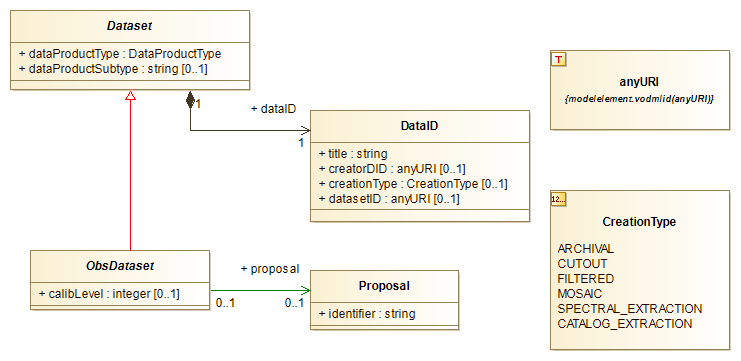
\includegraphics[width=0.9\textwidth]{notation_example.png}}
    \caption{Notation example diagram}\label{fig:notation_example}
  \end{center}
  \end{figure}

  \subsection{Class}
  \label{sect:Class}
  Classes are represented by a plain box that may be grouped in a package. The class name is annotated in the top window, abstract
classes use italic typeface. Attributes, if any, are listed in the lower panel. Attributes may only be
of primitive type (real, string, etc), a defined DataType, or an Enumeration type. Relationships to
other objects are defined via the composition and reference relation arrows.

  \subsection{DataType}
  \label{sect:DataType}
  DataTypes are represented by a box shape similar to Class, but annotated with a ``T'' symbol in the top left corner.

  \subsection{Enumerations}
  \label{sect:Enumerations}
  Enumerations are represented by a box shape similar to Class, but annotated with a ``1,2...''
symbol in the top left corner. Enumeration Literals (possible values) are listed below the
enumeration class name.

  \subsection{Generalization}
  \label{sect:Generalization}
  Generalizations are represented by a line (shown in red in Figure \ref{fig:notation_example}), with open triangle at the end of the source, or more general, object.

  \subsection{Composition}
  \label{sect:Composition}
  The composition relation is indicated by a line with a solid diamond attached to the
containing object, and an arrow pointing to the object being contained. The composition relation is
very tight, where the container is responsible for the creation and existence of the target. Any
object may be in no more than one composition relation with any container. The attribute name
for the composition relation is annotated at the destination of the relation (e.g., ``+ dataID''). This is
typically a lower-cased version of the destination class name, but this is not required.

  \subsection{Reference}
  \label{sect:Reference}
  The reference relation is indicated by a line (shown in green in Figure \ref{fig:notation_example}), with an arrow pointing to the object being
referenced. The reference relation is much looser than composition, the container has no
ownership of the target, but merely holds a pointer, or other indirect connection to it. The
attribute name is annotated at the destination of the relation (e.g., ``+ proposal''). This is typically
a lower-cased version of the destination class name, but may be another name indicating the role
that the class is playing in this context.

  \subsection{Multiplicity}
  \label{sect:Multiplicity}
  All attributes and relations have a multiplicity associated with them. For attributes, the multiplicity
is contained within brackets just after the attribute name. If no bracket is displayed, this is
equivalent to '[1]'.
\begin{itemize}
\item 1 = one and only one value must be provided.
\item 0..1 = zero or one value may be provided.
\item * = zero or more values may be provided (open ended).
\end{itemize}

  \subsection{Subsetted role}
  \label{sect:Subset}
Subsetted role constraints are shown in diagrams as a UML constraint of type $<<Subset>>$. The value of a subsetted property is restricted to the specified sub-type of that given in the parent class (see also Section 2.41 in \citet{2018ivoa.spec.0910L}).
